\documentclass[oneside,a4paper,13pt]{book}

\usepackage[a4paper,inner = 1.7cm, outer = 2.7cm, top = 2cm, bottom = 2cm, bindingoffset = 1.2cm]{geometry}
\usepackage[french]{babel}
\usepackage{blindtext}
\usepackage[utf8]{inputenc} 
\usepackage[T1]{fontenc}
\usepackage{graphicx}

\usepackage{microtype}
\usepackage{graphicx}
\usepackage{amsmath}
\usepackage{amssymb}
\usepackage{index}
\usepackage{titlesec}
\usepackage{siunitx}

\sisetup{detect-all = true}

\titleformat{\chapter}[display]
  {\Huge\bfseries}
  {}
  {0pt}
  {\thechapter.\ }
  
 \titleformat{name=\chapter,numberless}[display]
  {\Huge\bfseries}
  {}
  {0pt}
  {}

\begin{document}

\title{%
	BE Physique - Rayonnement thermique \\
	\large Pertes thermiques dans l'habitat et isolation}
	
\author{Nicolas Servot}
\date{Lundi 11 mai 2020}

\maketitle
\tableofcontents

\chapter{Conduction}
\section{Les murs d'habitation}

\paragraph{Question 1} 
\textit{Annoter le schéma avec les différents transferts thermiques entre les atmosphères intérieur et extérieur, le sens du flux thermique et les températures principales caractéristiques.} \\* 

\begin{figure}[h!]
\centering
  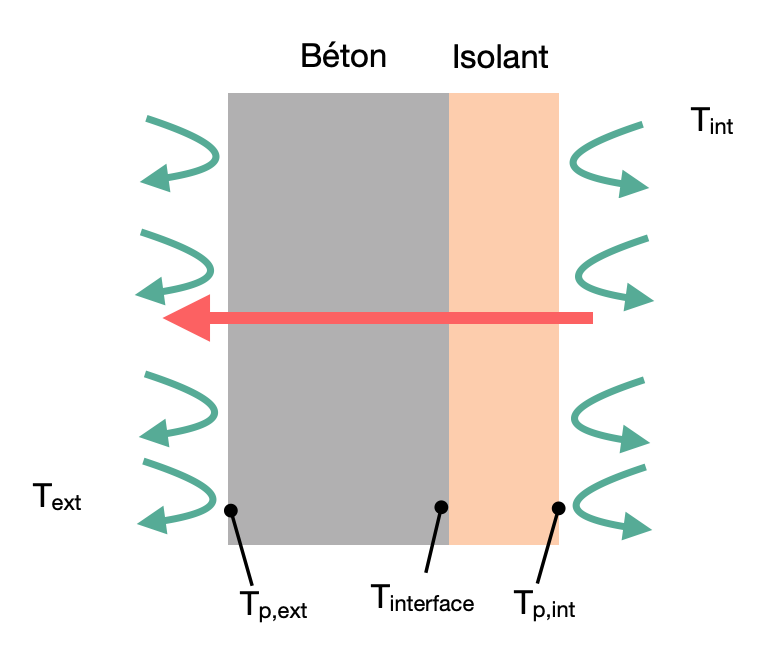
\includegraphics[width=0.5\linewidth]{q1.png}
  \caption{Transfert de chaleur. En rouge: conduction, en vert: convection.}
  \label{fig:q1}
\end{figure}

\paragraph{Question 2} 
\textit{Calculer la résistance thermique globale entre les deux températures connues pour\SI{1}{ \meter\squared} de surface de mur.} \\* 

La thermorésistance du mur prend en compte les effets conductifs et convéctifs. L'association de béton et d'isolant étant en série, on a  :

\begin{equation} \label{eq1}
\begin{split}
	R_{total} & = R_{conv} + R_{conduc} \\
	& = \frac{1}{h_{e} S} +  \frac{1}{h_{i} S} +  \frac{e_{isolant}}{\lambda_{isolant} S} + \frac{e_{beton}}{\lambda_{beton} S} \\
	& = \SI{2.8}{\kelvin\per\watt}
\end{split}
\end{equation}

\paragraph{Question 3} 
\textit{Calculer le flux de chaleur traversant un tel mur.}  

\begin{equation} \label{eq2}
\begin{split}
	\varphi & = \frac{T_{int} - T_{ext}}{R_{total}} \\
	& = \SI{6.0}{\watt}
\end{split}
\end{equation}

\paragraph{Question 4} 
\textit{Calculer les températures de paroi interne, externe et d’interface isolant mur.} 

En notant $T_{interface}$ la température à l'interface, $T_{p}^{ext}$ la température du mur extérieur et  $T_{p}^{int}$ la température du mur intérieur, on a :

%\begin{equation} \label{eq3}
\begin{gather}
	\varphi = S h_{i} (T_{int} - T_{p}^{int}) \Leftrightarrow T_{p}^{int} = T_{int} - \frac{\varphi}{S h_{i}}   \implies   T_{p}^{int} = \SI{18.4}{\celsius} \\
	\varphi = S h_{e}  (T_{p}^{ext} - T_{ext}) \Leftrightarrow T_{p}^{ext} = T_{ext} + \frac{\varphi}{S h_{e}} \implies   T_{p}^{ext} = \SI{2.6}{\celsius} \\
	\varphi = \frac{S \lambda_{beton}}{e_{beton}} (T_{p}^{int} - T_{interface}) + \frac{S \lambda_{isolant}}{e_{isolant}} (T_{p}^{ext} - T_{interface}) \implies T_{interface} = \SI{3.4}{\celsius}
\end{gather}
%\end{equation}

\paragraph{Question 5} 
\textit{Nous venons de voir le cas d’une isolation par l’intérieur, quelles seraient les pertes thermiques si le mur était isolé par l’extérieur ? Qu’en est-il des profils de températures dans les matériaux constituant le mur ? Que vous inspirent ces résultats ?} \\*

Dans ce cas, les résultats trouvés par les equations (1.3) et (1.4) restent inchangés. Seule l'équation (1.6) est modifiée  :

\begin{gather}
	\varphi = \frac{S \lambda_{isolant}}{e_{isolant}} (T_{p}^{int} - T_{interface}) + \frac{S \lambda_{beton}}{e_{beton}} (T_{p}^{ext} - T_{interface}) \implies T_{interface} = \SI{17.6}{\celsius}
\end{gather}

Dans les deux cas, les échanges thermiques sont equivalents. En effet, les gradients de température dans les 2 matériaux sont inchangés comme on peut le voir sur le profil de température.

\begin{figure}[h!]
\centering
  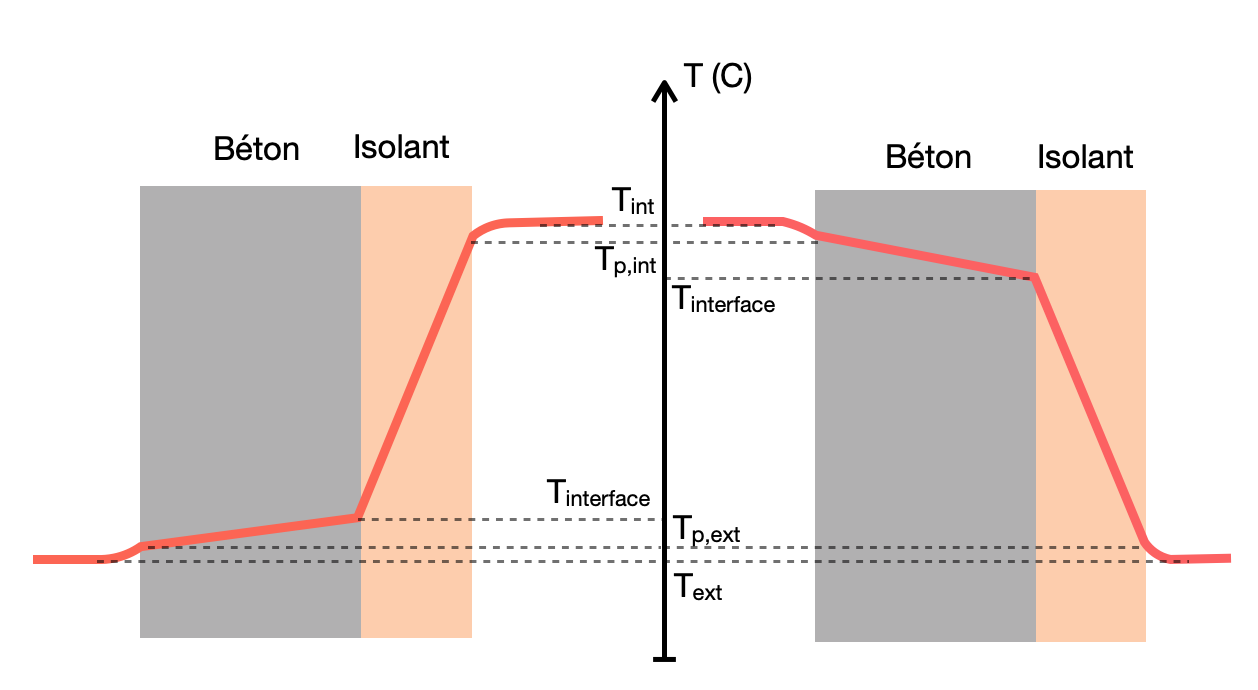
\includegraphics[width=0.9\linewidth]{q5.png}
  \caption{Profil de température. A gauche: 1e option, a droite: 2e option}
  \label{fig:q5}
\end{figure}

Les deux processus d'isolement sont equivalents, cependant on préfèrera la première option afin de protéger l'isolant de l'extérieur.

\newpage

\paragraph{Question 6} 
\textit{Annoter le schéma avec les différents transferts thermiques entre les atmosphères intérieur et extérieur, le sens du flux thermique et les températures principales caractéristiques.} 

\begin{figure}[h!]
\centering
  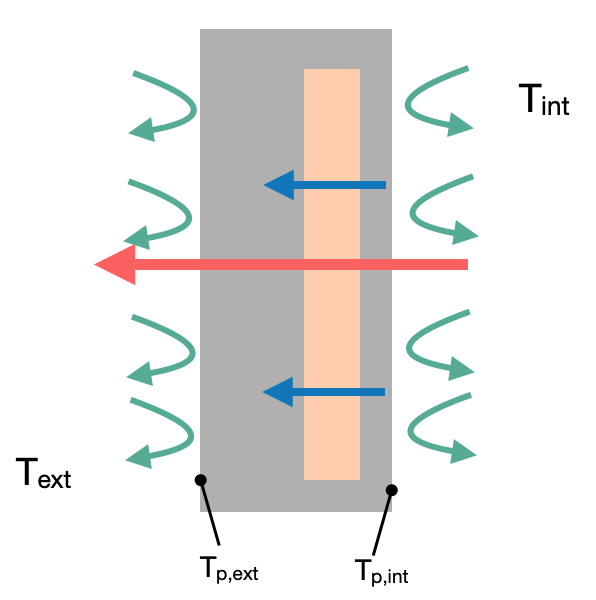
\includegraphics[width=0.4\linewidth]{q6.png}
  \caption{Transfert de chaleur. En rouge et bleu: conduction, en vert: convection}
  \label{fig:q1}
\end{figure}

\paragraph{Question 7} 
\textit{Calculer la résistance thermique globale entre les deux températures connues et pour une telle structure.} \\* \\*

On fixe la longueur du mur à 1m.
Dans le cas d'une association en parallèle, on a 

\begin{equation} \label{eq7}
\begin{split}
	\frac{1}{R_{parallele}} & = \frac{1}{R_{isolant}} + \frac{1}{R_{beton}^{sup}} + \frac{1}{R_{beton}^{inf}} \\
	& = \frac{\lambda_{isolant} S_{isolant}}{e_{isolant}} + 2 \frac{\lambda_{beton} S_{beton}}{e_{beton}} \\
	& = \SI{7.0}{\watt\per\kelvin}
\end{split}
\end{equation}

Finalement, 

\begin{equation} \label{eq8}
\begin{split}
	R_{total} & = R_{parallele} + R_{mur interieur} + R_{mur structure} + R_{convection} \\
	& = R_{parallele} +  \frac{e_{beton}}{\lambda_{beton} S_{mur}} + \frac{2}{h S_{mur}} \\
	& = \SI{0.26}{\kelvin\per\watt}
\end{split}
\end{equation}

\paragraph{Question 8} 
\textit{Calculer le flux de chaleur traversant une telle structure.} 

\begin{equation} \label{eq9}
\begin{split}
	\varphi & = \frac{T_{int} - T_{ext}}{R_{total}} \\
	& = \SI{65}{\watt}
\end{split}
\end{equation}

\paragraph{Question 9} 
\textit{Pour comparer avec le mur précédant, exprimer le flux de par\SI{}{ \meter\squared} de section de transfert.} 

\begin{equation} \label{eq10}
\begin{split}
	\Phi_{surfacique} & = \frac{\varphi}{S_{mur}} \\
	& = \SI{23}{\watt}
\end{split}
\end{equation}


\paragraph{Question 10} 
\textit{Finalement quelle préconisation pouvez-vous faire concernant l’isolation d’un bâtiment ?} \\* 

En normalisant le flux, on s'aperçoit que $\Phi_{surfacique} > \varphi$, ce qui s'explique notament par le manque d'isolation au sol. Ainsi, il est préférable de procéder comme dans le premier cas afin d'isoler au mieux sa maison.

\newpage
\section{Calorifuger les canalisations d'eau chaude d'une habitation}

\paragraph{Question 11} 
\textit{Annoter le schéma avec les différents transferts thermiques entre les atmosphères intérieur et extérieur, le sens du flux thermique.} \\* \\*

\begin{figure}[h!]
\centering
  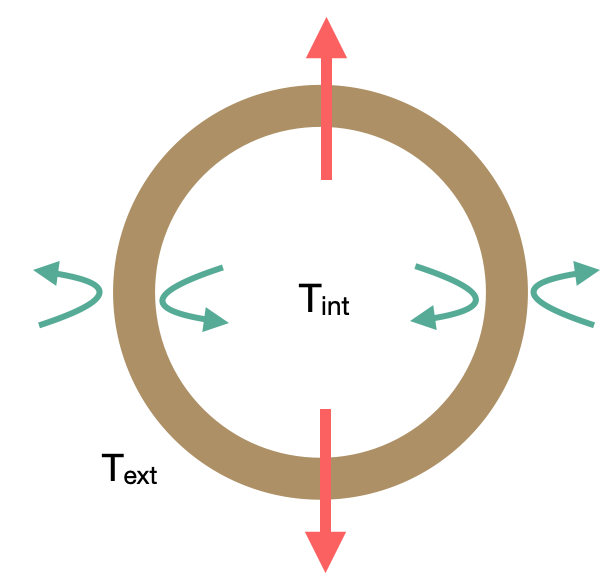
\includegraphics[width=0.5\linewidth]{q11.png}
  \caption{Transfert de chaleur. En rouge: conduction, en vert: convection.}
  \label{fig:q11}
\end{figure}

\paragraph{Question 12} 
\textit{ Calculer la résistance thermique globale entre les deux températures connues pour\SI{1}{ \meter} de canalisation.} \\* 

Posons $R_{cuivre}$ la thermorésistance du cuivre, et déterminons son expression puis sa valeur. On fixe la longueur $L$ du tube a 1m.\\* \\*
La loi de Fourier affirme

\begin{equation} \label{eq11}
\begin{split}
	\vec{j_{th}} & =  -\lambda_{cuivre} \vec{grad}(T) \\
	& = -\lambda_{cuivre} \frac{\partial T}{\partial r} \vec{u_{r}}
\end{split}
\end{equation}

Par définition du flux thermique, on a

\begin{equation} \label{eq11}
\begin{split}
	\varphi & =  \int \vec{j_{th}}\dot\ \vec{dS} \\
	& = \int j_{th} dS_{lateral}\\
	& = j_{th} L2\pi r
\end{split}
\end{equation}

En injectant (1.11) dans (1.12), on a

\begin{gather}
	\varphi  =  -\lambda_{cuivre} \frac{\partial T}{\partial r} L 2\pi r \\
	\Rightarrow \Delta T = \frac{\varphi}{\lambda_{cuivre}L2\pi} \ln{\frac{r_{2}}{r_{1}}}
\end{gather}

Par identification, on trouve

\begin{equation} \label{eq15}
\begin{split}
	R_{cuivre} & = \ln{\frac{r_{2}}{r_{1}}}\frac{1}{\lambda_{cuivre}L2\pi} \\
	& = \SI{76}{\micro\kelvin\per\watt}
\end{split}
\end{equation}

Finalement, la thermorésistance totale $R_{totale}$ vaut

\begin{equation} \label{eq12}
\begin{split}
	R_{total} & = R_{convection}^{int} + R_{convection}^{ext} + R_{cuivre} \\
	& = \frac{1}{h_{int}2 \pi L r_{1}} + \frac{1}{h_{ext}2 \pi L r_{2}} +  \ln{\frac{r_{2}}{r_{1}}}\frac{1}{\lambda_{cuivre}L2\pi} \\
	& = \SI{3.0}{\kelvin\per\watt}
\end{split}
\end{equation}

\paragraph{Question 13} 
\textit{ Calculer le flux de chaleur perdu par m linéaire de canalisation.} \\* \\*

\begin{equation} \label{eq17}
\begin{split}
	\Phi_{lineique} & = \frac{\varphi}{L} \\
	& = \frac{\Delta T}{L R_{total}} \\
	& = \SI{23}{\watt\per\meter}
\end{split}
\end{equation}

\paragraph{Question 14} 
\textit{ Devant de telle perte, le tube est enveloppé d’un isolant d’épaisseur\SI{1}{ \milli\meter} et de conductivité thermique $\lambda_{\mathrm{isolant}}$ =\SI{0.1}{\watt\per\meter\per\kelvin} (très inférieur au cuivre). Quel est alors le flux thermique perdu dans ce cas par mètre linéaire de canalisation isolée.} \\*

Par un raisonement analogue a la question 13, on peut exprimer $R_{total}$ comme

\begin{equation} \label{eq12}
\begin{split}
	R_{total} & = R_{convection}^{int} + R_{convection}^{ext} + R_{cuivre} + R_{isolant} \\
	& = \frac{1}{h_{int}2 \pi L r_{1}} + \frac{1}{h_{ext}2 \pi L (r_{2} + e_{isolant})} +  \ln{\frac{r_{2}}{r_{1}}}\frac{1}{\lambda_{cuivre}L2\pi} + \frac{1}{h_{ext}L2\pi (r_{2} + e_{isolant})} \\
	& = \SI{2.8}{\kelvin\per\watt}
\end{split}
\end{equation}

La flux linéique $\Phi_{lineique}$ s'écrit alors comme

\begin{equation} \label{eq17}
\begin{split}
	\Phi_{lineique} & = \frac{\varphi}{L} \\
	& = \frac{\Delta T}{L R_{total}} \\
	& = \SI{25}{\watt\per\meter}
\end{split}
\end{equation}

\paragraph{Question 15} 
\textit{Pouvez-vous faire une préconisation concernant l’isolation d’un tel tube ?} \\* \\*

De toute évidence, ajouter une couche d'isolant n'a pas l'effet escompté. Au contraire, par ce procédé le flux linéique est plus élevé qu'avant. Cela s'explique notament pas le fait que la surface de contact entre le tuyau et l'exterieur a été augmenté, on augmente ainsi les pertes thermiques. \\*

La solution serait d'isoler de l'intérieur, ce qui n'est pas idéal puisque cela diminue le débit d'eau dans la conduite. De plus, il faudrait traiter l'isolant pour limiter ses interactions avec l'eau.  \\*

Une autre solution serait de choisir un isolant plus performant afin de diminuer son épaisseur.

\end{document}
